% Final paper, laid out like the course's IEEE template
% (project-template-letter.docx). Build the PDF from the docs/ folder with:
%     pdflatex paper.tex   (run it twice so table and figure numbers resolve)
% Every number comes from results/ and figures/, produced by
%     python3 -m experiments.run_all --workers 6
% Red text marks details only the authors can fill in.

\documentclass[10pt,twocolumn,letterpaper]{article}
\usepackage[margin=0.75in,columnsep=0.25in]{geometry}
\usepackage{mathptmx}          % Times font, like the IEEE template
\usepackage[T1]{fontenc}
\usepackage{graphicx}
\usepackage{booktabs}
\usepackage{enumitem}
\usepackage{xcolor}
\usepackage{caption}
\usepackage{titlesec}
\usepackage[hidelinks]{hyperref}

% IEEE-style headings: I. INTRODUCTION, A. Subsection
\renewcommand\thesection{\Roman{section}}
\renewcommand\thesubsection{\Alph{subsection}}
\titleformat{\section}{\centering\normalsize\scshape}{\thesection.}{0.5em}{}
\titleformat{\subsection}{\normalsize\itshape}{\thesubsection.}{0.5em}{}
\titlespacing*{\section}{0pt}{1.2ex}{0.8ex}
\titlespacing*{\subsection}{0pt}{1ex}{0.5ex}
\captionsetup[table]{labelformat=simple,labelsep=newline,font={footnotesize,sc},
  justification=centering}
\renewcommand\thetable{\Roman{table}}
\captionsetup[figure]{font=footnotesize,name=Fig.,labelsep=period}

\graphicspath{{../figures/}}
\newcommand{\fillin}[1]{\textcolor{red}{[#1]}}

\title{\Large Search versus Simulation: Comparing Minimax and\\ Monte Carlo Tree Search in Connect Four}
\author{
  \begin{tabular}{c@{\hspace{3em}}c}
  Jonah Femiani & Ryan Hogan \\
  College of Engineering and Computing & College of Engineering and Computing \\
  Miami University & Miami University \\
  Oxford, Ohio & Oxford, Ohio \\
  femianjy@miamioh.edu & hoganrj@miamioh.edu \\
  \end{tabular}}
\date{}

\begin{document}
\maketitle

\noindent\textbf{\textit{Abstract}---Board games give a clear, measurable setting for
comparing how artificial intelligence methods plan ahead. To demonstrate, we built 
multiple agents for Connect Four. The first uses depth-limited minimax search with a hand-written 
evaluation function and alpha-beta pruning. The second uses Monte Carlo tree search, which needs 
no evaluation function and instead judges moves by playing many random games. We tested both against a
random agent and a greedy agent, and against each other, over 3440 games while varying how
deep each agent searches. Both agents beat the baselines almost every time once given
modest search: minimax from a depth of two moves and Monte Carlo tree search from 300
iterations. We also analyzed how Alpha-beta pruning reduced the positions minimax examined (at depth six) by 97.5
percent, making it 59 times faster without changing any move. Head to head, minimax was
stronger when both agents had the same time per move, winning 69 percent of games averaging
40 milliseconds per move, while Monte Carlo tree search caught up only when given almost five
times as much processing time.}

\medskip
\noindent\textbf{\textit{Keywords}---game playing, adversarial search, minimax, alpha-beta
pruning, Monte Carlo tree search, Connect Four}

\section{Introduction}

Connect Four is a two-player game played on a board seven columns wide and six rows tall.
Players will take turns dropping pieces into a column, and the first to line up four pieces
horizontally, vertically, or diagonally wins. The game is simple enough to program in an
afternoon but has far too many positions and gamestates to be able to solve by brute force, this makes it
a perfect setting for studying adversarial search~[1]. With optimal play, the first player
can always force a win~[2], but finding those moves in real time will force us to implement some smarter searches.

The two classic approaches to this kind of search operate very differently. \emph{Minimax}~[1]
looks a fixed number of moves ahead and relies on a hand-written evaluation function to
score positions it cannot see to the end, we also implement \emph{alpha-beta pruning}~[3]. This makes it faster
without changing its decisions by avoiding unnecessary searches. \emph{Monte Carlo tree search} (MCTS)~[4],~[5] needs no
evaluation function: it estimates how good each move is by playing many random games to the
end, focusing its effort on the moves that offer the best outcomes. We will go more in depth as
to the specifics of how they work later. Comparing them shows the trade-off between relying on 
human game knowledge and relying on raw simulation.

Our goal was to compare these two methods on the same game. Specifically, we asked:
\begin{enumerate}[leftmargin=*,nosep]
  \item How does each agent's win rate change as it is allowed to search more (deeper for
        minimax, more iterations for MCTS), against random and greedy opponents?
  \item Which method plays better head to head, and at what cost in time per move?
  \item How much does alpha-beta pruning reduce the work minimax does?
\end{enumerate}

First we implemented a basic rendition of the game, then two baseline agents, and both AI agents in Python. We then ran 3,440
simulated games with fixed random seeds. Both agents beat the baseline agents almost every time once search depth surpassed two moves. 
We also noticed Alpha-beta pruning cut the positions searched at depth 6 by 97.5\%.
Head to head, minimax won more often when both agents had the same time per move, but MCTS
improved steadily with more iterations and matched or beat minimax when given about five
times more time.

\section{Methodology}

\subsection{Data and Preprocessing}

This project does not use an external dataset. Instead, data was generated through the games played
between agents. We ran 44 matchups: 32 of 100 games each and 12 of 20 games each (explained in Section~II-C), for 3,440 games in total. Within
each matchup, the two agents alternate who moves first, because the first player has an
advantage in Connect Four~[2]. Every game uses its own fixed random seed, derived from a base
seed of 42, so any game can be replayed exactly (rerunning matchups produced identical game
outcomes).

For each game we record the winner (or a draw), the number of moves, and for each agent its
settings (search depth or iterations), the time it spent calculating per move, and for minimax we also tracked the
number of positions it searched. There is no training step, so no train and test split is
needed and there is no risk of possible data leakage. The minimax evaluation function and the MCTS
settings were chosen by hand before the experiments and were not tuned on the games we
report.

\subsection{AI Model and Implementation}

\textit{Game representation.} The board is stored as a six-by-seven grid in which each cell
is empty or holds one player's piece. After every move, the program checks only the lines
passing through the newly placed piece, since a new win must include that piece.

\textit{Baseline agents.} The \emph{random agent} chooses uniformly among the legal
columns. The \emph{greedy agent} plays a winning move if one exists, otherwise blocks the
opponent's immediate win if one exists, and otherwise plays randomly.

\textit{Minimax agent.} Minimax~[1] explores the tree of possible future moves to a fixed
depth. It assumes the agent picks the move with the highest score and the opponent picks the
move with the lowest. Won and lost positions get very large positive or negative scores,
adjusted by the remaining depth so that faster wins and slower losses are preferred.
Positions at the depth limit are scored by an evaluation function that looks at all 69
groups of four cells in a line on the board. Each group holding three of the agent's pieces
and one empty cell adds 5 points, and each with two pieces and two empty cells adds 2,
the same patterns for the opponent subtract the same amounts. Groups containing both
players' pieces can never become a win and score nothing. Finally, each piece in the center
column adds 3 points for its owner, because the center column is part of the most possible
lines of four.

\textit{Alpha-beta pruning.} Alpha-beta pruning~[3] keeps track of the best score each
player is already guaranteed elsewhere in the tree, and stops exploring a branch as soon as
it is clear that a sensible player would never allow it. It always returns the same move as
plain minimax but usually searches far fewer positions. Our implementation can switch
pruning on or off, so the two versions can be compared directly. Moves are tried from the
center column outwards, which tends to find good moves early and lets pruning skip more
branches.

\textit{MCTS agent.} MCTS~[4],~[5] builds a search tree gradually. Each iteration has four
steps. \emph{Selection} walks down the tree from the current position, at each step choosing
the move with the highest Upper Confidence Bound (UCB1) score~[4]. UCB1 adds a move's
win rate so far to a bonus that is large for moves tried only a few times, balancing
promising moves against unexplored ones, we use the standard exploration constant of
$\sqrt{2}$. \emph{Expansion} adds one untried move to the tree. \emph{Simulation} plays
random moves from that position until the game ends. \emph{Backpropagation} updates the
visit and win counts of every node on the path back to the root, counting a draw as half a
win. After all iterations, the agent plays the move that was visited most, which is more
reliable than the move with the highest win rate, since a rarely visited move may just have
been lucky.

\textit{Tools.} The project is written in Python 3~[6]. The game and agents use only the
standard library, and figures are made with Matplotlib~[7]. Per Python, all requirements can
be found in "requirements.txt".

\textit{Generative AI Disclosure} Along the development of this project we utilized tools
like used Claude Code and GitHub Copilot. The use of these tools helped us with general debugging
by building unit tests, along with adding further documentation to our code.

\subsection{Experimental Setup}

We ran four experiments, all with a base seed of 42:
\begin{enumerate}[leftmargin=*,nosep]
  \item \emph{Minimax strength.} Minimax with pruning, at depths 1 through 6, played 100
        games against each baseline.
  \item \emph{MCTS strength.} MCTS with 100, 300, 1,000, 3,000, and 5,000 iterations
        played 100 games against each baseline.
  \item \emph{Head to head.} Minimax at depths 2, 4, and 6 played 100 games against MCTS
        with 100, 1,000, and 5,000 iterations.
  \item \emph{Cost of pruning.} Minimax without pruning, at depths 1 through 6, played 20
        games against each baseline. Because pruning never changes minimax's moves, these
        games are move-for-move identical to the first 20 games of the pruned runs, which we
        confirmed, they serve only to measure search cost, so 20 games were enough.
\end{enumerate}
As a check on the baselines, the greedy agent also played 100 games against the random
agent.

\textit{Metrics.} \emph{Win rate} is the fraction of games won, with draws and losses
reported separately, it measures playing strength. With 100 games, a win rate near 50\% has
a 95\% confidence interval of about $\pm$10 percentage points, so smaller differences should
not be read as meaningful. \emph{Positions searched per move} counts the board positions
minimax examines before choosing a move; it measures computational effort and does not
depend on hardware. \emph{Time per move}, in milliseconds (ms), is the average time an agent
takes to choose a move, it is the only cost measure that applies to both methods, but it
depends on hardware.

\textit{Hardware.} All experiments ran on an Intel Core Ultra 7 155H processor (22 logical
cores) under Windows Subsystem for Linux 2 (WSL2) with Python 3.12.3. To save time, six matchups
ran in parallel, each in its own process (to avoid the Global Interpreter Lock), the full run 
took about 11.5 minutes. Running in parallel does not affect any game outcome, but it adds
some noise to the timings, which should be read as approximate.

\section{Experimental Results}

\begin{table*}[t]
\caption{Win / draw / loss rates (\%) of each agent against the baselines, and mean time per move}
\label{tab:baselines}
\centering\footnotesize
\begin{tabular}{llccr}
\toprule
Agent & Setting & vs.\ Random (W / D / L) & vs.\ Greedy (W / D / L) & ms per move \\
\midrule
Minimax & depth 1 & 100 / 0 / 0 & 69 / 0 / 31 & 0.18 \\
Minimax & depth 2 & 99 / 0 / 1 & 99 / 0 / 1 & 0.43 \\
Minimax & depth 3 & 100 / 0 / 0 & 100 / 0 / 0 & 1.65 \\
Minimax & depth 4 & 100 / 0 / 0 & 100 / 0 / 0 & 4.28 \\
Minimax & depth 5 & 100 / 0 / 0 & 100 / 0 / 0 & 18.98 \\
Minimax & depth 6 & 100 / 0 / 0 & 100 / 0 / 0 & 41.62 \\
\midrule
MCTS & 100 iterations & 100 / 0 / 0 & 85 / 2 / 13 & 4.37 \\
MCTS & 300 iterations & 100 / 0 / 0 & 98 / 0 / 2 & 13.42 \\
MCTS & 1,000 iterations & 100 / 0 / 0 & 98 / 0 / 2 & 46.93 \\
MCTS & 3,000 iterations & 100 / 0 / 0 & 100 / 0 / 0 & 147.31 \\
MCTS & 5,000 iterations & 100 / 0 / 0 & 99 / 1 / 0 & 252.90 \\
\midrule
Greedy & --- & 96 / 0 / 4 & --- & 0.05 \\
\bottomrule
\end{tabular}
\end{table*}

\begin{figure}[t]
\centering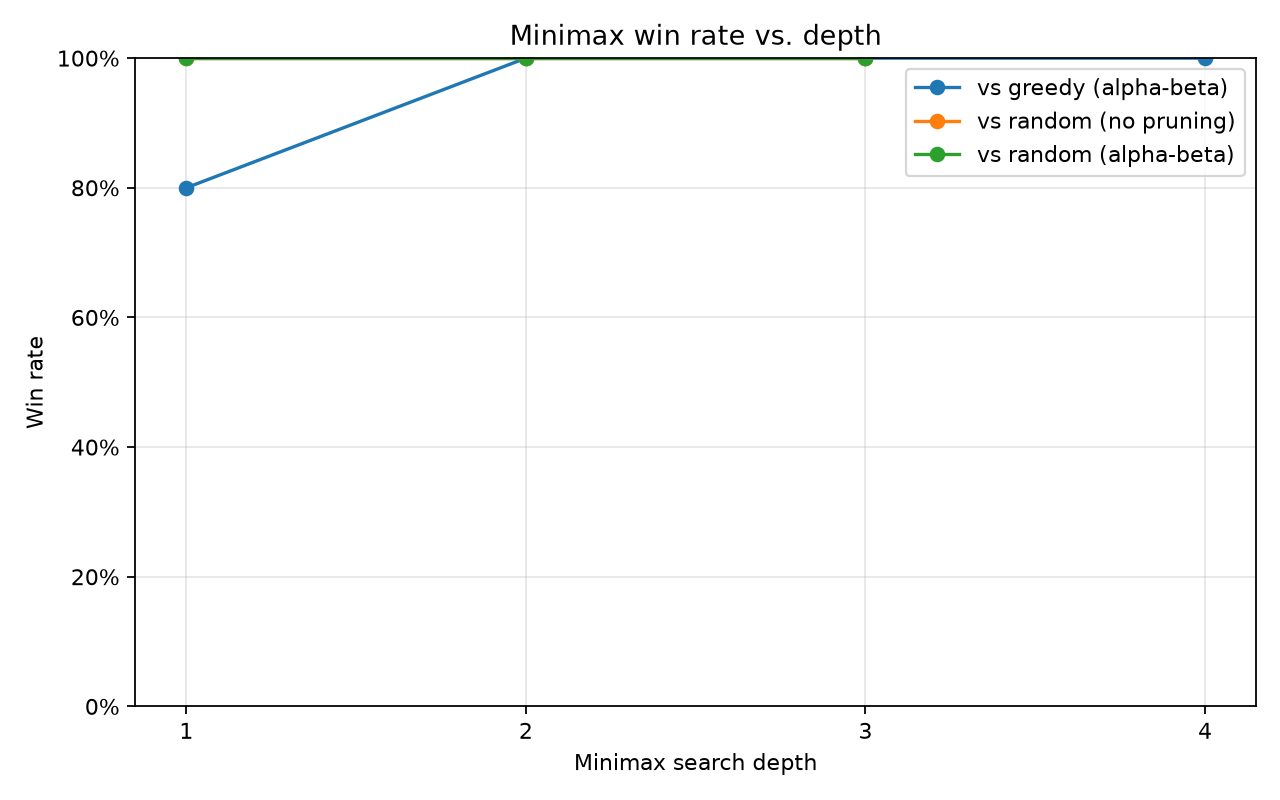
\includegraphics[width=\columnwidth]{win_rate_vs_depth.png}
\caption{Win rate (\%) of the minimax agent (with alpha-beta pruning) versus search depth,
against the random and greedy agents. 100 games per point.}
\label{fig:minimax}
\end{figure}

\begin{figure}[t]
\centering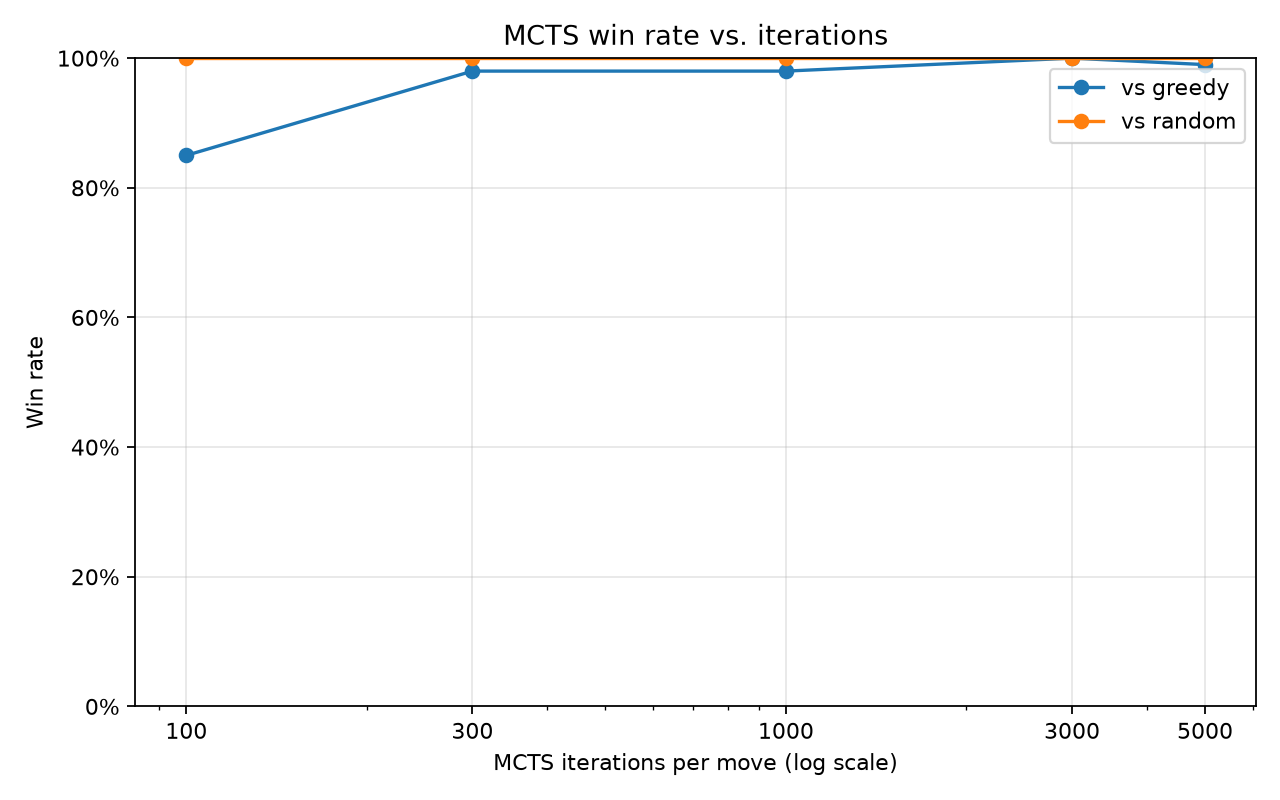
\includegraphics[width=\columnwidth]{win_rate_vs_iterations.png}
\caption{Win rate (\%) of the MCTS agent versus iterations per move (log scale), against the
random and greedy agents. 100 games per point.}
\label{fig:mcts}
\end{figure}

\subsection{Strength Against the Baselines}

Table~\ref{tab:baselines} lists every agent's results against the two baselines. The greedy
agent beat the random agent in 96\% of games, confirming that it is the stronger baseline.

Minimax (Fig.~\ref{fig:minimax}) beat the random agent at every depth, but at depth 1 it won
only 69\% of games against the greedy agent. At depth 1, minimax scores the position right
after its own move without looking at the opponent's reply. It always takes an immediate
win, but it notices the opponent's threats only indirectly, through the evaluation
function's penalty for the opponent's open three-in-a-rows, and that penalty is not always
enough to make it block. The greedy agent exploits the threats it leaves open. From depth 2, minimax sees the opponent's
immediate replies and blocks them, and it won 99\% of games. Its single loss to each
baseline at depth 2 is consistent with the horizon effect: a double threat, where the
opponent threatens two wins at once, takes three moves to see coming. From depth 3 onward,
minimax won every game.

MCTS (Fig.~\ref{fig:mcts}) also beat the random agent every time, even with only 100
iterations. Against the greedy agent, it won 85\% of games at 100 iterations, with 13
losses and 2 draws. With 100 iterations spread over up to seven moves, each move gets only
about 14 random playouts, too few to reliably notice an immediate threat. From 300
iterations onward, MCTS won 98--100\% of games.

\begin{table}[t]
\caption{Search cost of minimax with and without alpha-beta pruning (same 40 games per depth)}
\label{tab:pruning}
\centering\footnotesize
\begin{tabular}{crrrrr}
\toprule
& \multicolumn{2}{c}{Positions per move} & & \multicolumn{2}{c}{ms per move} \\
\cmidrule(lr){2-3}\cmidrule(lr){5-6}
Depth & Pruned & Unpruned & Saved & Pruned & Unpruned \\
\midrule
1 & 7 & 7 & 0.0\% & 0.28 & 0.25 \\
2 & 23 & 51 & 55.0\% & 0.42 & 1.12 \\
3 & 101 & 373 & 72.8\% & 1.91 & 6.59 \\
4 & 264 & 2,321 & 88.6\% & 3.99 & 46.29 \\
5 & 1,100 & 15,629 & 93.0\% & 18.97 & 312.77 \\
6 & 2,383 & 95,268 & 97.5\% & 36.49 & 2,148.38 \\
\bottomrule
\end{tabular}
\end{table}

\begin{figure}[t]
\centering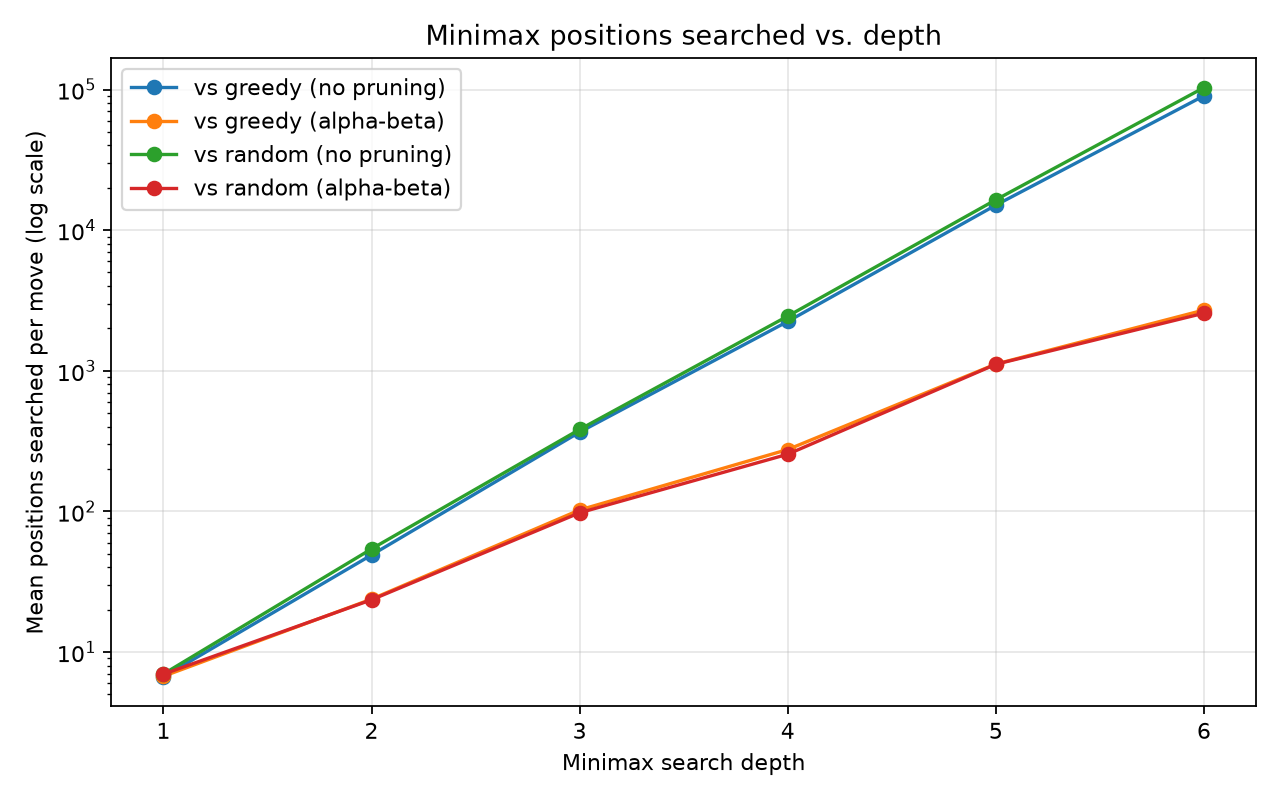
\includegraphics[width=\columnwidth]{positions_searched_vs_depth.png}
\caption{Mean positions searched per move by minimax versus search depth, with and without
alpha-beta pruning (log scale).}
\label{fig:positions}
\end{figure}

\begin{figure}[t]
\centering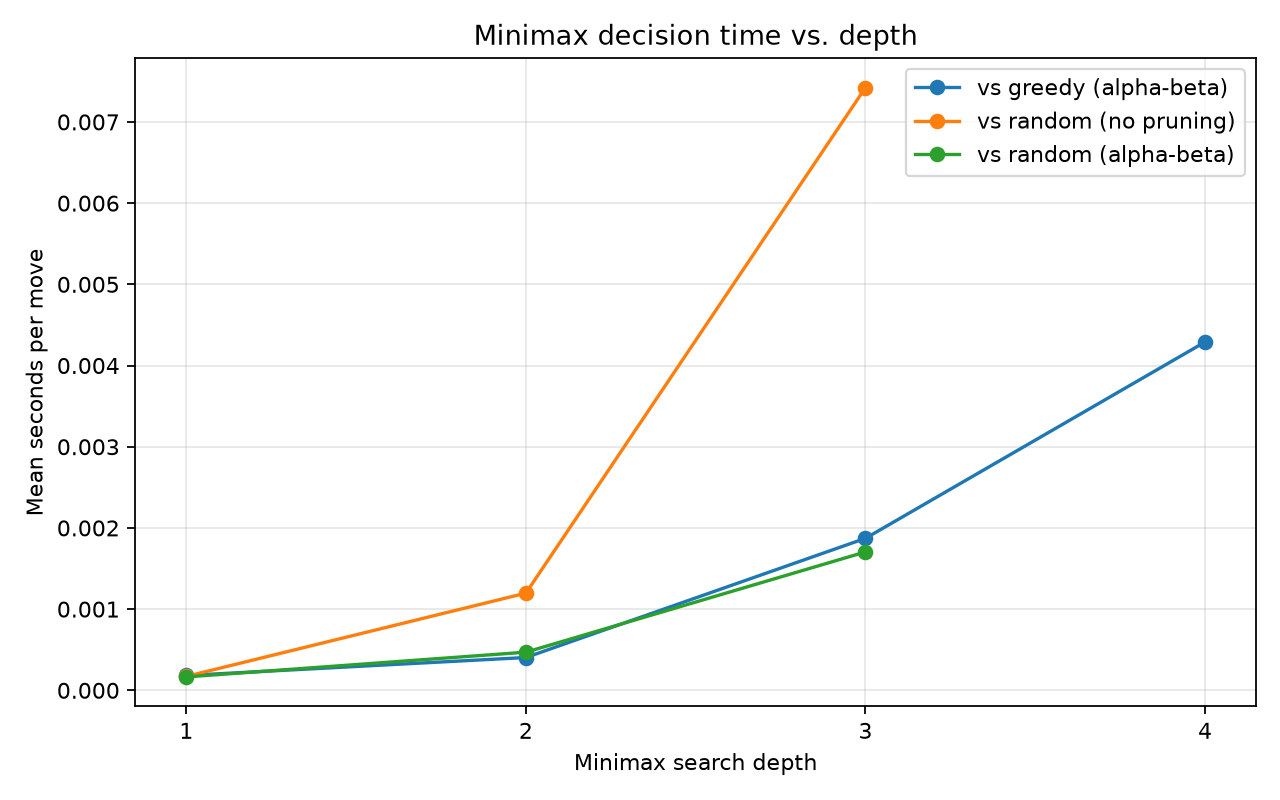
\includegraphics[width=\columnwidth]{time_per_move_vs_depth.png}
\caption{Mean time per move (s) of minimax versus search depth, with and without alpha-beta
pruning (log scale).}
\label{fig:time}
\end{figure}

\subsection{Cost of Search and the Effect of Pruning}

Table~\ref{tab:pruning} compares minimax with and without pruning on the same 40 games at
each depth (20 against each baseline). Both versions chose identical moves in every game,
as expected. Without pruning, the positions searched grew by a factor of about 6 to 7 per
extra move of depth (Fig.~\ref{fig:positions}), close to the 7 legal moves available in most
positions. With pruning, the growth was only about 2 to 4 times per extra move,
approaching the theoretical best case for alpha-beta pruning, a growth of roughly the square
root of the number of moves, or about 2.6~[3]. At depth 1 pruning saves nothing, because every position after one
move is scored immediately and there is nothing left to skip. At depth 6, pruning examined
97.5\% fewer positions and chose moves 59 times faster, about 36~ms instead of over 2~s.
Time per move followed the same pattern as positions searched (Fig.~\ref{fig:time}).

\begin{table}[t]
\caption{Minimax versus MCTS head to head: minimax win / draw / loss (\%) and mean time per move (ms)}
\label{tab:headtohead}
\centering\footnotesize
\begin{tabular}{lccc}
\toprule
& MCTS 100 & MCTS 1,000 & MCTS 5,000 \\
\midrule
Minimax depth 2 & 91 / 0 / 9 & 50 / 0 / 50 & 39 / 0 / 61 \\
Minimax depth 4 & 95 / 1 / 4 & 55 / 0 / 45 & 42 / 0 / 58 \\
Minimax depth 6 & 95 / 0 / 5 & 69 / 1 / 30 & 58 / 0 / 42 \\
\midrule
\multicolumn{4}{l}{Time per move: minimax depth 2, 4, 6: 0.4, 4.0, 37~ms.} \\
\multicolumn{4}{l}{MCTS 100, 1,000, 5,000 iterations: 4.6, 39, 190~ms.} \\
\bottomrule
\end{tabular}
\end{table}

\begin{figure}[t]
\centering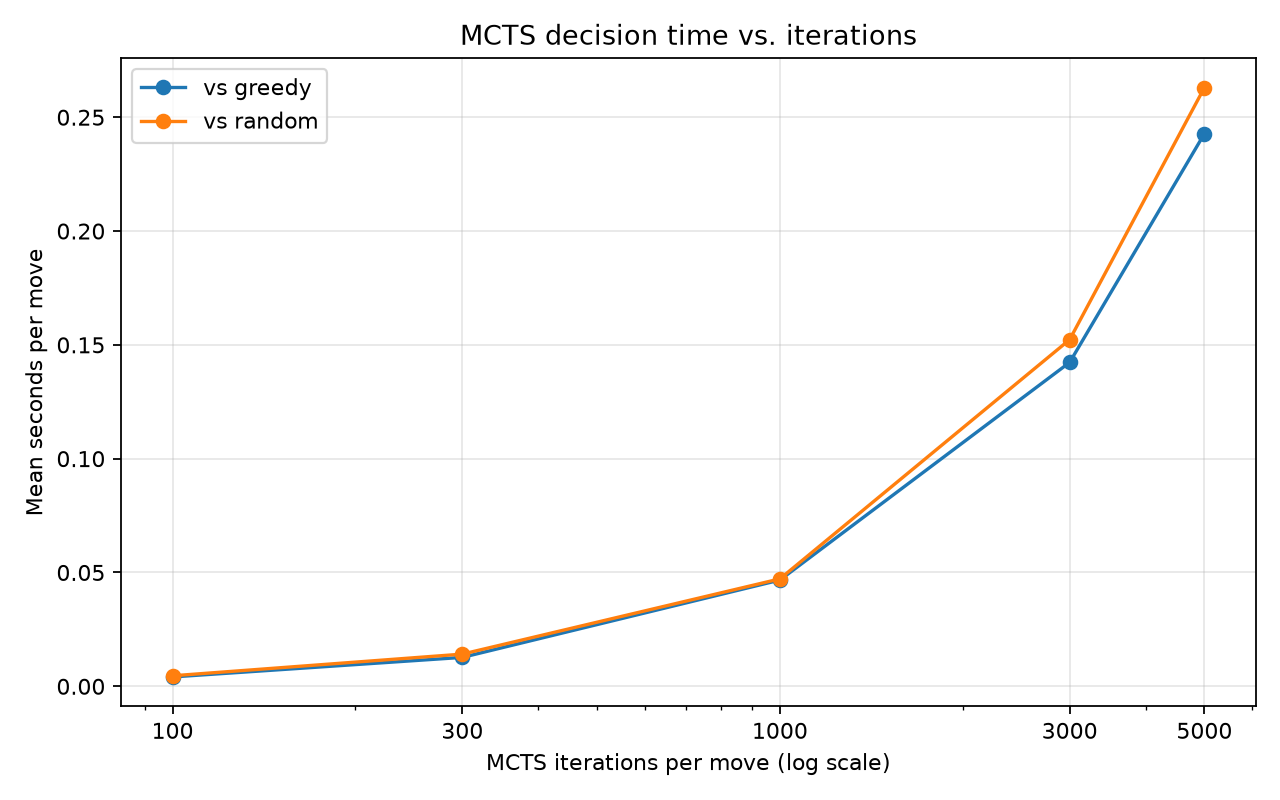
\includegraphics[width=\columnwidth]{time_per_move_vs_iterations.png}
\caption{Mean time per move (s) of MCTS versus iterations per move (log scale).}
\label{fig:mctstime}
\end{figure}

\subsection{Minimax versus MCTS}

Table~\ref{tab:headtohead} shows the head-to-head results. The fairest comparisons pair
settings that take about the same time per move. Minimax at depth 4 and MCTS with 100
iterations both take about 4 to 5~ms per move, and minimax won 95\% of games. Minimax at
depth 6 and MCTS with 1,000 iterations both take about 40~ms per move, and minimax won
69\%. For the same time, minimax was clearly stronger.

MCTS improved steadily with more iterations. Against minimax at depth 2, its win rate rose
from 9\% at 100 iterations to 50\% at 1,000 and 61\% at 5,000. With 5,000 iterations, MCTS
also won 58\% of games against minimax at depth 4, and minimax at depth 6 won only 58\% of
games against it, both results are within the margin of error of an even result. MCTS's time per move grows in proportion to
its iterations (Fig.~\ref{fig:mctstime}), about 0.05~ms per iteration, so this extra
strength cost about five times more time per move than minimax at depth 6.

Two results stand out. First, MCTS at 5,000 iterations beat minimax at depth 2 even though
minimax won at equal time per move. A likely reason is that MCTS's random playouts run all
the way to the end of the game, giving it a rough sense of long-term threats that a
two-move search cannot see. Second, increasing
minimax's depth from 2 to 6 helped much less against MCTS than against the baselines: its
win rate against MCTS with 1,000 iterations rose only from 50\% to 69\%, suggesting that the
hand-written evaluation function, not just the depth, limits how well minimax plays.

\section{Conclusion}

We built two Connect Four agents, one based on minimax search with alpha-beta pruning and
one based on Monte Carlo tree search, and compared them with each other and with random and
greedy baselines over 3,440 games. Both agents beat the baselines almost every time once
given modest search: minimax from depth 2 and MCTS from 300 iterations. Alpha-beta pruning
made minimax 59 times faster at depth 6 without changing any move. Head to head, minimax was
the stronger method for the same time per move, winning 69\% of games at about 40~ms per
move, while MCTS needed about five times as much time to reach an even result. We learned
that a small amount of game knowledge in an evaluation function goes a long way when time
is limited, while simulation-based search keeps improving with more time and needs no game
knowledge at all.

\textit{Limitations.} Our baselines are weak, and we did not test against strong or human
players. The minimax evaluation function and the MCTS settings were chosen by hand and not
tuned. Each matchup used 100 games, so differences of less than about 10 percentage points
near an even result are not meaningful. Timings depend on our hardware and Python's speed,
and they include some noise because six matchups ran in parallel.

\textit{Next steps.} Natural extensions are rerunning the timings one matchup at a time,
testing against a perfect-play solver, adding a transposition table so minimax can search
deeper, and giving MCTS smarter playouts than purely random moves. We could also experiment
with how the agents scale with larger board sizes.

\section*{References}
\begin{enumerate}[label={[\arabic*]},leftmargin=*,itemsep=2pt,font=\footnotesize]
\footnotesize
\item S. Russell and P. Norvig, \textit{Artificial Intelligence: A Modern Approach}, 4th ed.
  Hoboken, NJ: Pearson, 2020.
\item L. V. Allis, ``A knowledge-based approach of Connect-Four: The game is solved: White
  wins,'' M.S. thesis, Vrije Universiteit, Amsterdam, The Netherlands, 1988.
\item D. E. Knuth and R. W. Moore, ``An analysis of alpha-beta pruning,'' \textit{Artificial
  Intelligence}, vol. 6, no. 4, pp. 293--326, 1975, doi: 10.1016/0004-3702(75)90019-3.
\item L. Kocsis and C. Szepesv\'ari, ``Bandit based Monte-Carlo planning,'' in \textit{Proc.
  17th European Conf. Machine Learning (ECML)}, 2006, pp. 282--293, doi: 10.1007/11871842\_29.
\item C. B. Browne \textit{et al.}, ``A survey of Monte Carlo tree search methods,''
  \textit{IEEE Trans. Computational Intelligence and AI in Games}, vol. 4, no. 1, pp. 1--43,
  2012, doi: 10.1109/TCIAIG.2012.2186810.
\item Python Software Foundation, ``Python 3 documentation.'' [Online]. Available:
  \url{https://docs.python.org/3/}
\item J. D. Hunter, ``Matplotlib: A 2D graphics environment,'' \textit{Computing in Science
  \& Engineering}, vol. 9, no. 3, pp. 90--95, 2007, doi: 10.1109/MCSE.2007.55.
\end{enumerate}

\end{document}
